\documentclass[theme=example,language=english]{hgbthesis}
\ExecuteBibliographyOptions{giveninits=true}
\addbibresource{references.bib}
\usepackage{bookmark}
% stub: tag macros (anonymised corpus)
\newcommand{\tagname}[1]{\texttt{<#1>}}
\newcommand{\attr}[1]{\texttt{#1}}

% stub: placeholder for sections without content yet
\newcommand{\placeholderemptysection}{\emph{This section is intentionally left empty.}}


\usepackage[section]{placeins}
\usepackage{listings}

# inspired by: https://tex.stackexchange.com/questions/10255/xml-syntax-highlighting
\definecolor{gray}{rgb}{0.35,0.35,0.35}
\definecolor{darkblue}{rgb}{0.0,0.0,0.65}
\definecolor{purple}{rgb}{0.51,0.0,0.95}

\lstset{basicstyle=\ttfamily,columns=fullflexible,showstringspaces=false,commentstyle=\color{gray}\upshape}

\lstdefinelanguage{XML}
{
    morestring=[b]",
    moredelim=[s][\bfseries\color{darkblue}]{<}{\ },
    moredelim=[s][\bfseries\color{darkblue}]{</}{>},
    moredelim=[l][\bfseries\color{darkblue}]{/>},
    moredelim=[l][\bfseries\color{darkblue}]{>},
    morecomment=[s]{<?}{?>},
    stringstyle=\color{purple}\textbf,
    identifierstyle=\color{darkblue},
    keywordstyle=\color{red},
    morekeywords={name, label, limits, data, size, unit, file}
}
\lstdefinelanguage{none}{
    identifierstyle=
}


\usepackage[strings]{underscore}
\usepackage{color}
\usepackage{multirow}
\usepackage{arydshln}
\usepackage[list=true]{subcaption}
\usepackage{amsmath}
\usepackage{tcolorbox}
\usepackage{longtable}
\usepackage{tikz}
\usetikzlibrary{shapes.geometric, arrows, angles}

% product name with registered sign
\newcommand{\ExampleSim}{ExampleSim\textsuperscript{\textregistered}}


\title{\ExampleSim\ Documentation}
\author{Author One \& Author Two \\ and many more}
\placeofstudy{ Institute of Examples \& Institute of Samples}

\begin{document}
\frontmatter
\maketitle
\tableofcontents
\mainmatter
\chapter{Introduction}\label{ch:intro}
\ExampleSim\ reads XML input files, see \autoref{sec:input} and \cite{knuth84}.
\section{Overview}\label{sec:overview}
\begin{figure}[htb]\centering
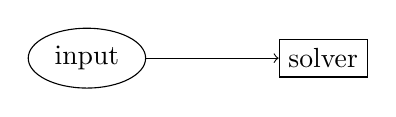
\begin{tikzpicture}\node[draw, ellipse] (a) {input}; \node[draw, rectangle] (b) at (3,0) {solver}; \draw[->] (a) -- (b);\end{tikzpicture}
\caption{Data flow}\label{fig:flow}\end{figure}
Identifiers like file_name and data_size use underscores.
\begin{tcolorbox}Note: see \autoref{fig:flow}.\end{tcolorbox}

\chapter{Usage}\label{ch:usage}
\section{Input files}\label{sec:input}
\begin{GenericCode}[language=XML]
<model name="example" file="a.xml">
  <data size="3" unit="m"/>
</model>
\end{GenericCode}
The tag \tagname{model} has the attribute \attr{name}.

% sub-chapter include: no chapter heading, joins the preceding compilation unit (A5)
\section{Details}\label{sec:details}
\begin{longtable}{ll}\caption{Parameters}\label{tab:params}\\\hline Name & Unit\\\hline\endfirsthead
\hline Name & Unit\\\hline\endhead
param_1 & m\\
param_2 & m\\
param_3 & m\\
param_4 & m\\
param_5 & m\\
param_6 & m\\
param_7 & m\\
param_8 & m\\
param_9 & m\\
param_10 & m\\
param_11 & m\\
param_12 & m\\
param_13 & m\\
param_14 & m\\
param_15 & m\\
param_16 & m\\
param_17 & m\\
param_18 & m\\
param_19 & m\\
param_20 & m\\
param_21 & m\\
param_22 & m\\
param_23 & m\\
param_24 & m\\
param_25 & m\\
param_26 & m\\
param_27 & m\\
param_28 & m\\
param_29 & m\\
param_30 & m\\
param_31 & m\\
param_32 & m\\
param_33 & m\\
param_34 & m\\
param_35 & m\\
param_36 & m\\
param_37 & m\\
param_38 & m\\
param_39 & m\\
param_40 & m\\
param_41 & m\\
param_42 & m\\
param_43 & m\\
param_44 & m\\
param_45 & m\\
\hline\end{longtable}
\placeholderemptysection

\chapter{Reference}\label{ch:reference}
\begin{table}[htb]\centering\caption{Options}\label{tab:opts}
\begin{tabular}{l:l}\hline \multirow{2}{*}{solver} & fast\\ & exact\\\hline\end{tabular}\end{table}
\begin{align} x &= \sum_{i=1}^n a_i \label{eq:sum}\end{align}
See \autoref{eq:sum}, \autoref{tab:params} and \cite{lamport94}.

\printbibliography
\end{document}
